%課題研究レジュメテンプレート ver. 1.2

\documentclass[uplatex]{jsarticle}
\usepackage[top=20mm,bottom=20mm,left=20mm,right=20mm]{geometry}
\usepackage[T1]{fontenc}
\usepackage{txfonts}
\usepackage{wrapfig}
\usepackage[expert,deluxe]{otf}
\usepackage[dvipdfmx,hiresbb]{graphicx}
\usepackage[dvipdfmx]{hyperref}
\usepackage{pxjahyper}
\usepackage{secdot}

\makeatletter
  \renewcommand{\section}{%
    \if@slide\clearpage\fi
    \@startsection{section}{1}{\z@}%
    {\Cvs \@plus.5\Cdp \@minus.2\Cdp}% 前アキ
    {.5\Cvs \@plus.3\Cdp}% 後アキ
    %{\normalfont\Large\headfont\raggedright}}
    {\normalfont\raggedright}}

  \renewcommand{\subsection}{\@startsection{subsection}{2}{\z@}%
    {\Cvs \@plus.5\Cdp \@minus.2\Cdp}% 前アキ
    {.5\Cvs \@plus.3\Cdp}% 後アキ
    %{\normalfont\large\headfont}}
    {\normalfont}}

  \renewcommand{\subsubsection}{\@startsection{subsubsection}{3}{\z@}%
    {\Cvs \@plus.5\Cdp \@minus.2\Cdp}%
    {\z@}%
    %{\normalfont\normalsize\headfont}}
    {\normalfont}}
\makeatother
%ここから上を編集する必要はない.





\title{\vspace{-14mm}Redpenを使った文書自動添削ツール}
\author{PMコース 矢吹研究室 1442031 氏名 小山 隆太郎}
\date{}%日付を入れる必要はない.
\pagestyle{empty}%ページ番号は振らない.
\begin{document}
\maketitle





\section{研究の背景}
ソフトウェアエンジニアはプログラムを組むだけではなく,たくさんの技術文書を書く.そして専門的なチュートリアル,マニュアル等を読み手に理解してもらうことが大切である.ソフトウェアを開発する際には多くの実装テストをする必要がある.そのためCheckStyleやlint等の静的解析ツールを導入することで,フォーマットのエラーを自動で検知することが出来る.しかし静的解析ツールは文書のチェックを行えるものがなく,文中のミスを修正することに時間を割く等で作業の本質に取り組む時間以外に無駄が生じてしまうことがある.このような状況に対してRedpenと呼ばれる文書静的解析ツールが開発され,日々エンジニアが改良を加えている\cite{a}.Redpenは一部の静的解析ツール(CheckStyle,lint等)に相当する機能を文書に与えるものであり,文書作成でも最低限の検査を自動で行いたいという動機の下,改良が進んでいる.大学の授業等で文書を提出することがあるため,Redpenの開発に着目することでこれからの文書作成の質が向上するのではないかと考えた.

\section{研究の目的}
Redpenを利用し,文書作成に割く時間を短縮できるようにすることで,もっと大きな粒度の問題(実作業,着目すべき文や質等)に集中できるようにすることが目的である.また,文中のミスを少なくした状態で文書を提出できるようにする\cite{b}.そのため,仮想環境上でRedPenが動作するよう設定を行う.

\section{研究の手法}
\begin{itemize}
 \item1.Redpenが動作する環境を仮想環境を用いて構築する\cite{c}.
 \item2.参考文献のサンプル文\cite{d}とWebページからの引用文等で添削を行い,添削結果が本の改善文に準拠するよう設定ファイルを書き換える.
 \item3.研究概要文をRedPenで添削しながら作成する.
\end{itemize}

\section{研究の結果}
本研究は以下のように進んでいる.
\begin{itemize}
 \item 1.RedPenを仮想環境で起動した.
 \item 2.RedPenの設定を編集し,添削機能を確立した.
\end{itemize}

\subsection{研究概論の添削結果}

執筆段階の本概論をRedPenで添削したところ,以下の文中ミスが指摘された.
\begin{itemize}
 \item FrequentSentenceStart:同じ文頭が連続して使用されている場合に指摘される.本概論の文頭に「RedPen」を過度に使用したため指摘された.
 \item JapaneseAmbiguousNounConjunction:名詞前後の接続詞が不要であることを指摘する.「文章の間の句点」を「文書間の句点」に修正したことで解消されたが,この文中ミスの指摘が一番多かった.
 \item SuccesiveWord:同一単語が連続して使用されている場合に指摘される.文中に「マシンをを」と間違えたまま添削したからである.
 \item InvalidSymbol:設定通りではない句点が使用されている場合に指摘される.句点を半角で入力していたため指摘された.
\end{itemize}
この段階で計11箇所の文中ミスが指摘された.指摘箇所を修正した結果3件に文中ミスを減らすことが出来た.

指摘箇所が残った原因として,設定が曖昧であることが考えられる.「文章の間の句点」を文中ミスで指摘しているが,「...の...の...」というパターンも文中ミスとして添削してしまう.例として,「私の研究室のパソコン」という文を,文中ミスとして指摘してしまう.

\subsection{引用文の添削結果}
参考文献\cite{d}の一文を以下に引用する.
\begin{quote}
 野菜ジュースは濃度が上がるほど食物繊維が豊富になりますが,嚥下機能の低下した人が誤嚥する危険が増えますが、そこで濃度の異なる野菜ジュースを作り、食物繊維の摂取量、安全、嗜好を考慮するとどの濃度が適切なのかを研究している.
\end{quote}

図1に引用文を添削した結果を載せる.

%\begin{wrapfigure}[行数]{r}{幅}%行数はオプションだが,調整しないとうまくいかない.
\begin{figure}[htb]
\centering
%\vspace*{-\intextsep}
%\includegraphics[width=図の幅,clip]{ファイル名}\label{参照用ラベル}
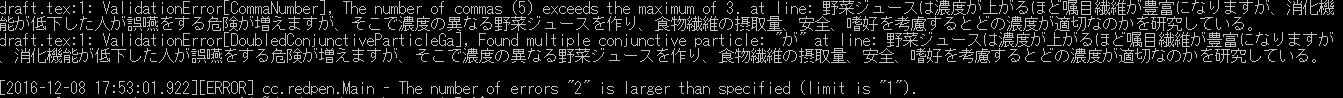
\includegraphics[width=16cm,clip]{image1.png}
\caption{引用文の添削結果}\label{サンプル図}
\end{figure}

\begin{itemize}
 \item DoubledConjunctiveParticleGa:一文に2回以上,接続助詞の「が」が検出されると二重否定になるため検出される.この場合「野菜ジュースは濃度が上がるほど食物繊維が豊富になりますが、消化機能が低下した人が誤嚥をする危険が増えますが、」と内容が理解しにくくなる.参考文献の改善案では,二重否定の片方を「です。」で閉じるべきと指摘し,この通りに文書を書き換え再度添削した結果,指摘は出力されなかった.
 \item CommaNumber:文中の句点の数が必要以上である場合に指摘される.この場合「濃度の異なる野菜ジュースを作り、食物繊維の摂取量、安全、嗜好を考慮するとどの濃度が適切なのかを研究している。」中の「摂取量、安全、嗜好」の句点を「・」にすることが技術文章では相応しい.
\end{itemize}


\subsection{考察}
RedPenには設定ファイルが設けられており,設定を書き換えるごとに出力結果も変わるため,きちんとした設定が確立されてなく,現状の機能は不十分である..Redpenのファイル設定を確立し,文中のミスを抽出することは出来たが,中には正しい文中表記が間違いであることを指摘された.添削を正確に行うためには,設定ファイルを粒度の細かい部分まで作成する必要があると考察する.

\section{今後の計画}
RedPenの設定を見直した上で,RedPen導入後の文書の質と書く時間の変化を調査する予定である.

\bibliographystyle{junsrt}
\bibliography{biblio}%「biblio.bib」というファイルが必要.

\end{document}
